\chapter{Resultados, Discussões e Trabalhos Futuros}
	\label{capituloFinal}
	
	Em posse da técnica descrita no capítulo \ref{capituloReconstrucao} e dos \textit{softwares} expostos no capítulo \ref{capituloSoftwares}, foi possível obter resultados com certo grau de corretude e com grande potencial de melhora em sua exatidão.
	
	A seguir são apresentados testes, resultados e discussões acerca das atividades desenvolvidas neste trabalho.
	
	\section{Testes validadores}
		\label{secaoTestes}
		
		Como descrito no capítulo \ref{materiaisEMetodos}, a corretude da técnica desenvolvida, e consequente validade dos resultados obtidos, foi aferida através de cenas específicas (figura \ref{cenasValidacao}) cujos dados foram catalogados previamente.
		
		Após alguns testes preliminares, com valores para a tolerância projetiva igual a $3$ e incremento igual a $0.002$, todas as cenas de validação obtiveram seus mais adequados resultados; dependo, individualmente, apenas do critério arbitrário de convergência.
		
		Para a cena de validação 1 (figura \ref{cenaValidacao1}), cuja montagem de dados está expressa na figura \ref{printTesteCubo}, o melhor critério de convergência foi o de valor de coordenada Z mais próximo ao anteriormente analisado. Demorando, em média, seis minutos e dez segundos para concluir, a reconstrução da cena de validação 1 retornou os dados da tabela \ref{tabelaErrosCubo}.
		
		\begin{table}
			\caption{Dados da reconstrução da cena de validação 1}
			\label{tabelaErrosCubo}
			\begin{center}
				\begin{tabular}{r r r | r r r | r}
					\hline
					\multicolumn{3}{c}{Obtido} & \multicolumn{3}{c}{Desejado}\\
					\cline{1-6}
					\multicolumn{1}{c}{X} & \multicolumn{1}{c}{Y} & \multicolumn{1}{c}{Z} & \multicolumn{1}{c}{X} & \multicolumn{1}{c}{Y} & \multicolumn{1}{c}{Z} & \multicolumn{1}{c}{Erro geométrico}\\
					\hline			
					0.00625				&			0.007035714		&		0				&		0		&		0		&		0		&		0.009410833\\
					0.996142857		&			0.003428571		&		0				&		1		&		0		&		0		&		0.005160683\\
					0.992					&			0.990393443		&		0				&		1		&		1		&		0		&		0.012501438\\
					0.005571429		& 		0.994571429		&		0				&		0		&		1		&		0		&		0.007778831\\
					0.995111111		&			0.005407407		&		0.99		&		1		&		0		&		1		&		0.012375027\\
					0.997					&			0.998					&		0.99		&		1		&		1		&		1		&		0.010630146\\
					0.010571429		&			0.017492063		&		0.99		&		0		&		0		&		1		&		0.022753624\\
					0.009538462		&			0.995461538		&		0.99		&		0		&		1		&		1		&		0.014545786\\
					\hline
				\end{tabular}
			\end{center}
		\end{table}
		
		Na cena de validação 2 (figura \ref{cenaValidacao2}), cuja montagem de dados é a da figura \ref{printTestePiramide}, o critério de convergência mais eficaz, por sua vez, foi o de valor de coordenada Z mais próximo à média dos valores possíveis. Com uma demora média para conclusão de quatro minutos, a reconstrução da cena 2 retornou os dados da tabela \ref{tabelaErrosPiramide}.
		
		\begin{table}
			\caption{Dados da reconstrução da cena de validação 2}
			\label{tabelaErrosPiramide}
			\begin{center}
				\begin{tabular}{r r r | r r r | r}
					\hline
					\multicolumn{3}{c}{Obtido} & \multicolumn{3}{c}{Desejado}\\
					\cline{1-6}
					\multicolumn{1}{c}{X} & \multicolumn{1}{c}{Y} & \multicolumn{1}{c}{Z} & \multicolumn{1}{c}{X} & \multicolumn{1}{c}{Y} & \multicolumn{1}{c}{Z} & \multicolumn{1}{c}{Erro geométrico}\\
					\hline			
					0.007					&			0.005					&		0.008		&		0			&		0			&		0		&		0.01174734\\
					0.011866667		&			0.99352				&		0.008		&		0			&		1			&		0		&		0.01571013\\
					0.9675671			&			0.989264069		&		0.008		&		1			&		1			&		0		&		0.035087793\\
					0.982966292		& 		0.004876404		&		0.008		&		1			&		0			&		0		&		0.019440332\\
					0.766722973		&			0.517574324		&		0.904		&		0.5		&		0.5		&		1		&		0.284017607\\
					\hline
				\end{tabular}
			\end{center}
		\end{table}
		
		Na cena de validação 3 (figura \ref{cenaValidacao3}) - montagem da figura \ref{printTesteCuboReduzido}, novamente, o critério de escolher coordenadas Z cujo valor é mais próximo ao plano analisado anteriormente foi o melhor. Em média, eram gastos seis minutos e vinte segundos para a reconstrução da cena de validação 3 retornar os dados da tabela \ref{tabelaErrosCuboReduzido}.
		
		\begin{table}
			\caption{Dados da reconstrução da cena de validação 3}
			\label{tabelaErrosCuboReduzido}
			\begin{center}
				\begin{tabular}{r r r | r r r | r}
					\hline
					\multicolumn{3}{c}{Obtido} & \multicolumn{3}{c}{Desejado}\\
					\cline{1-6}
					\multicolumn{1}{c}{X} & \multicolumn{1}{c}{Y} & \multicolumn{1}{c}{Z} & \multicolumn{1}{c}{X} & \multicolumn{1}{c}{Y} & \multicolumn{1}{c}{Z} & \multicolumn{1}{c}{Erro geométrico}\\
					\hline			
					0.507521739		&			0.512478261		&		0				&		0.5			&		0.5			&		0			&		0.014569954\\
					0.504075949		&			0.992075949		&		0				&		0.5			&		1				&		0			&		0.008910889\\
					0.989418182		&			0.511109091		&		0				&		1				&		0.5			&		0			&		0.01534232\\
					0.98727027		& 		0.981310811		&		0				&		1				&		1				&		0			&		0.022612647\\
					0.521545455		&			0.521545455		&		0.492		&		0.5			&		0.5			&		0.5		&		0.031502591\\
					0.511					&			0.99575				&		0.492		&		0.5			&		1				&		0.5		&		0.01425\\
					0.9972 				&			0.5164				&		0.492		&		1				&		0.5			&		0.5		&		0.018460769\\
					0.996181818		&			0.995454545		&		0.492		&		1				&		1				&		0.5		&		0.009961911\\
					\hline	
				\end{tabular}
			\end{center}
		\end{table}	
		
		\begin{figure}[!htb]
			\centering
			\subfloat[Panorama para a reconstrução da cena de validação 1]{
				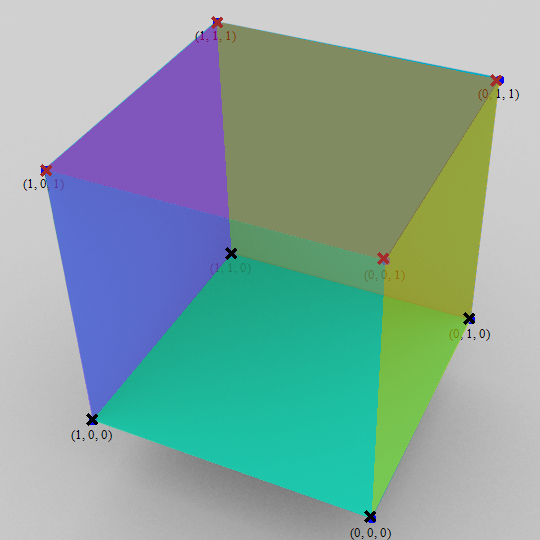
\includegraphics[height=4.5cm]{imagens/printTesteCubo.png}
				\label{printTesteCubo}
			}
			\quad
			\subfloat[Panorama da reconstrução da cena de validação 2]{
				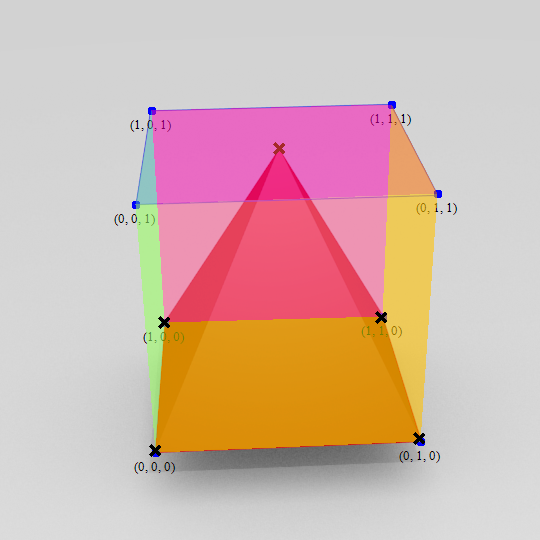
\includegraphics[height=4.5cm]{imagens/printTestePiramide.png}
				\label{printTestePiramide}
			}
			\quad
			\subfloat[Panorama da reconstrução da cena de validação 3]{
				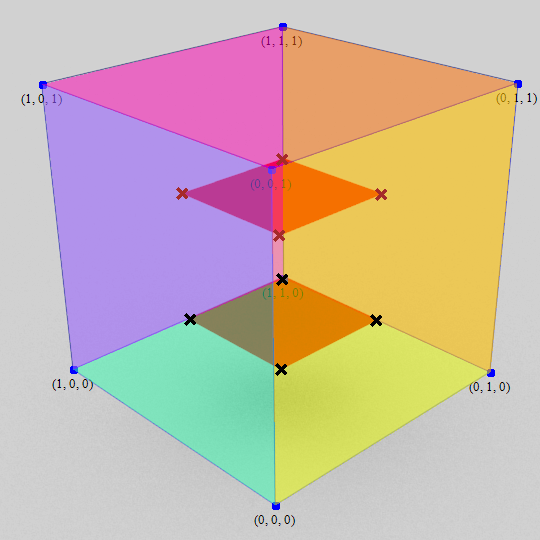
\includegraphics[height=4.5cm]{imagens/printTesteCuboReduzido.png}
				\label{printTesteCuboReduzido}
			}
			\caption{Panoramas das reconstruções de validação}
			\label{printTestes}
		\end{figure}
		
		Nota-se que, mesmo com certo erro numérico, a geometria dos objetos reconstruídos é mantida (figura \ref{printTestesMeshLab}); resguardando, ainda, certa proporção que tem sua exatidão afetada pelas aproximações (aproximação durante calibração e tolerância projetiva) efetuadas pela técnica de reconstrução.
		
		\begin{figure}[!htb]
			\centering
			\subfloat[Reconstrução da cena 1]{
				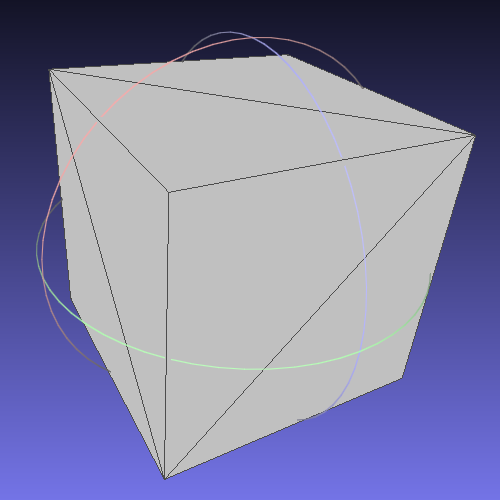
\includegraphics[height=4.5cm]{imagens/printTesteCuboMeshLab.png}
				\label{printTesteCuboMeshLab}
			}
			\quad
			\subfloat[Reconstrução da cena 2]{
				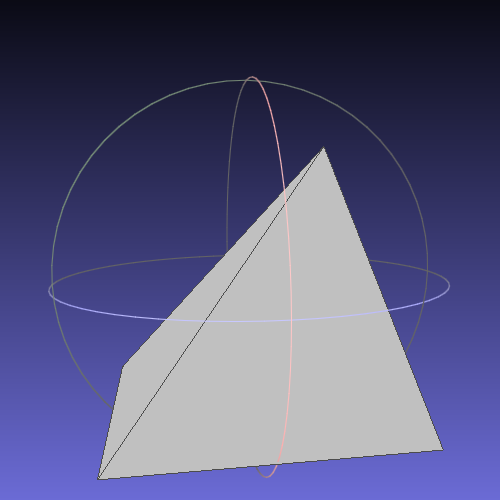
\includegraphics[height=4.5cm]{imagens/printTestePiramideMeshLab.png}
				\label{printTestePiramideMeshLab}
			}
			\quad
			\subfloat[Reconstrução da cena 3]{
				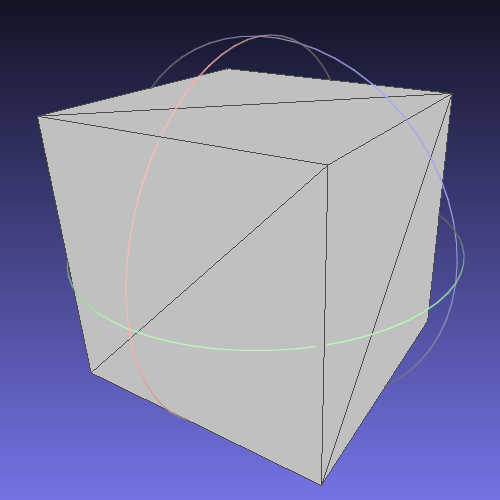
\includegraphics[height=4.5cm]{imagens/printTesteCuboReduzidoMeshLab.png}
				\label{printTesteCuboReduzidoMeshLab}
			}
			\caption{Reconstruções validadoras (faces inseridas manualmente)}
			\label{printTestesMeshLab}
		\end{figure}
		
		O caso menos bem-sucedido é o da cena 2, onde o vértice da pirâmide, dada a arbitrariedade do critério de escolha do valor da coordenada Z, é reconstruído muito abaixo da sua posição real causando um deslocamento das coordenadas X e Y e, como consequência, a deformação da pirâmide reconstruída.
		
		Através da escolha manual, disponibilizada pelo aplicativo de reconstrução, de valores para as coordenadas Z, há um erro geométrico médio menor entre os pontos, fazendo com que a geometria dos objetos reconstruídos, principalmente da pirâmide da cena 2, seja mais verossímil. Todavia, a escolha manual é uma estratégia notavelmente brusca e, por isso, resolveu-se não discuti-la nesta monografia.
		
		Todos os dados e resultados dos testes validadores, inclusive os correspondentes à escolha manual, estão disponíveis em \url{https://github.com/ivancezanne/TCC/tree/master/App_Reconstrucao/Testes}.
		
		\section{Resultados}
			\label{secaoResultados}
			
			Após os testes validadores, nos quais a técnica de reconstrução se mostrou factível, buscou-se a reconstrução das imagens descritas na seção \ref{secaoConjuntoDeDados}. Nem todas as imagens foram possíveis de serem reconstruídas, no entanto, pôde-se obter certo resultado com as imagens do \textit{VW Beetle} de Sutherland e da litografia de Dürer.
			
			Utilizando a preparação exposta na figura \ref{printTesteFusca}, uma tolerância projetiva igual a $2$, um incremento de $0.002$ e escolha de coordenada Z mais próxima ao último valor analisado, a reconstrução dos pontos de interesse demarcados para a imagem do \textit{VW Beetle} de Sutherland encontram-se na figura \ref{resultadosFuscaTriplo}.
			
			\begin{figure}[!htb]
				\centering
				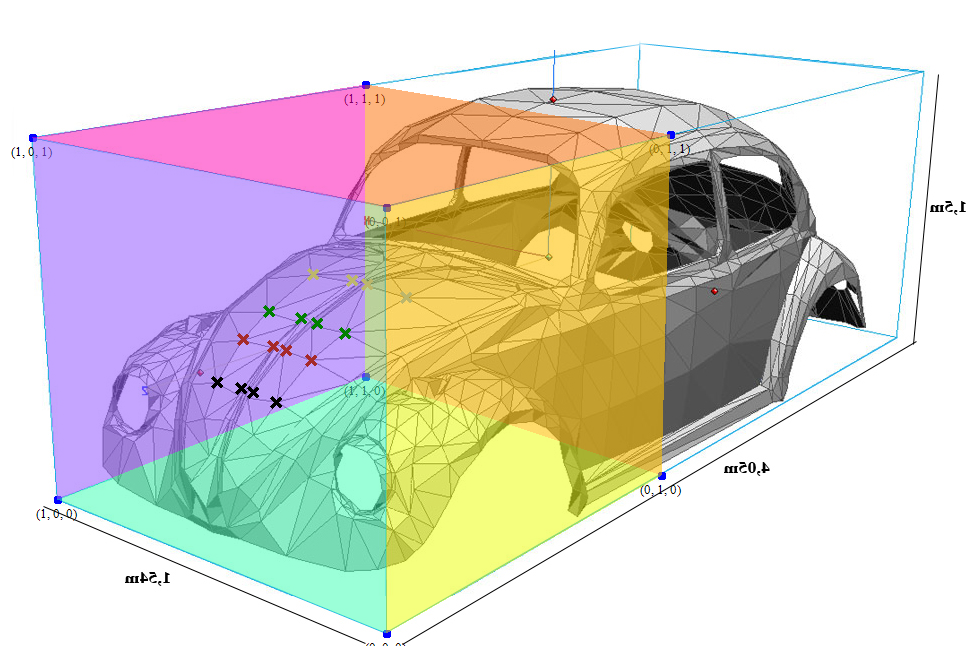
\includegraphics[height=9cm]{imagens/printTesteFusca.png}
				\caption{Panorama da reconstrução do \textit{VW Beetle} de Sutherland}
				\label{printTesteFusca}
			\end{figure}
			
			\begin{figure}[!htb]
				\centering
				\subfloat[Visão da lateral esquerda do \textit{VW Beetle} de Sutherland reconstruído]{
					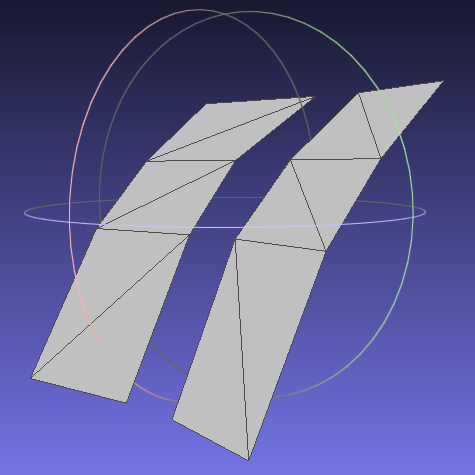
\includegraphics[height=4cm]{imagens/printResultadoFusca1.png}
					\label{resultadoFusca1}
				}
				\quad
				\subfloat[Visão frontal da reconstrução do \textit{VW Beetle} de Sutherland]{
					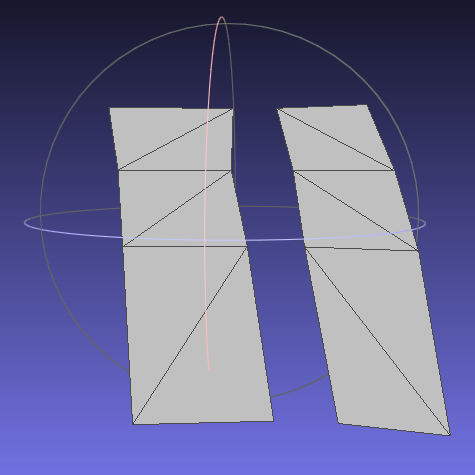
\includegraphics[height=4cm]{imagens/printResultadoFusca2.png}
					\label{resultadoFusca2}
				}
				\quad
				\subfloat[Visão da lateral direita do \textit{VW Beetle} de Sutherland reconstruído]{
					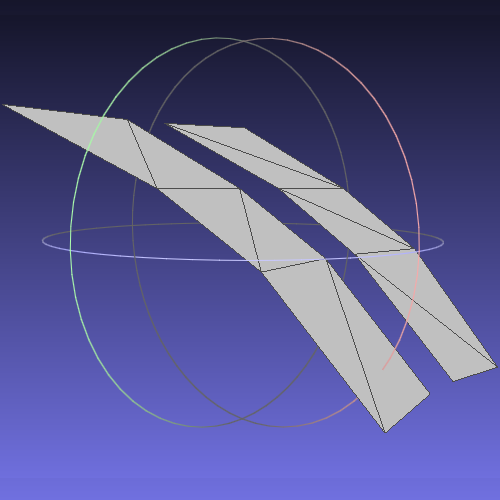
\includegraphics[height=4cm]{imagens/printResultadoFusca3.png}
					\label{resultadoFusca3}
				}
				\caption{A reconstrução do \textit{VW Beetle} de Sutherland (Faces inseridas manualmente)}
				\label{resultadosFuscaTriplo}
			\end{figure}
			
			Pela figura \ref{resultadosFuscaTriplo} nota-se que há certas deformações, uma vez que os segmentos de faces deveriam ser retilíneos quando vistos frontalmente. Todavia, nota-se o paralelismo entre os segmentos, o que é correto, além de esperado comportamento curvilíneo em relação ao eixo Z.
			
			De tal forma, conclui-se que a deformação é causada por um erro que ainda persiste na determinação das coordenadas Z. Tal erro se dá pois, além dos critérios finais de convergência serem arbitrários, eles, no máximo, seguem uma tendência de crescimento linear; ao passo que a curvatura (crescimento dos valores da coordenada Z para o capô do carro) segue um tendência próxima à logarítmica.
			
			Para a litografia de Dürer, a melhor configuração foi com tolerância projetiva igual a 3, incremento de 0.002 e escolha da coordenada Z mais próxima à média dos valore possíveis. Assim, com os dados para reconstrução expostos na figura \ref{printTesteDurer}, obtiveram-se os resultados da figura \ref{resultadosDurerTriplo}
			
			\begin{figure}[!htb]
				\centering
				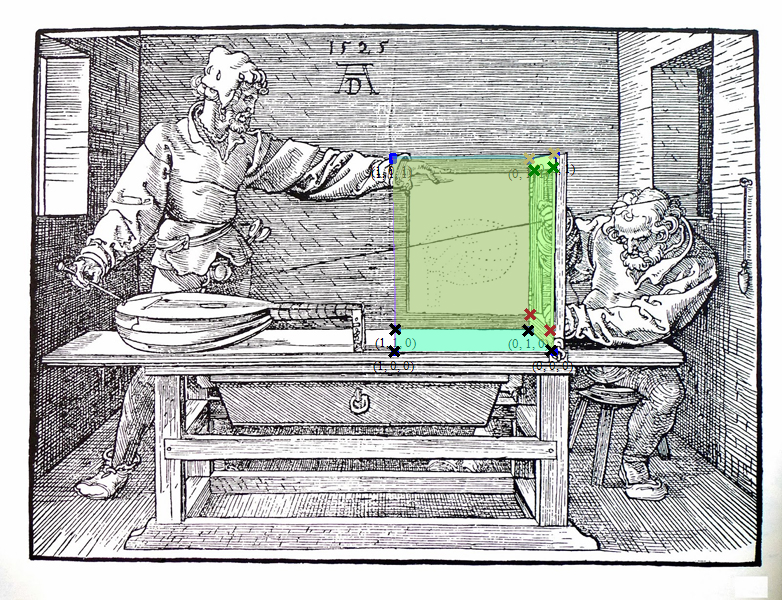
\includegraphics[height=10cm]{imagens/printTesteDurer.png}
				\caption{Panorama da reconstrução da litografia do Dürer}
				\label{printTesteDurer}
			\end{figure}
			
			\begin{figure}[!htb]
				\centering
				\subfloat[Reconstrução sob ponto de vista reverso em relação à cena da litografia de Dürer]{
					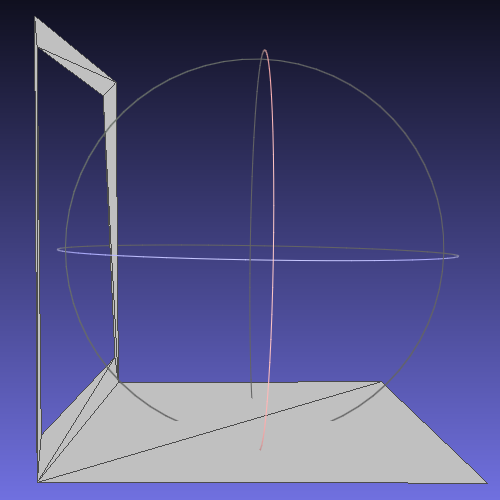
\includegraphics[height=4cm]{imagens/printResultadoDurerReverso.png}
					\label{resultadosDurer1}
				}
				\quad
				\subfloat[Reconstrução em vista lateral da cena da litografia de Dürer]{
					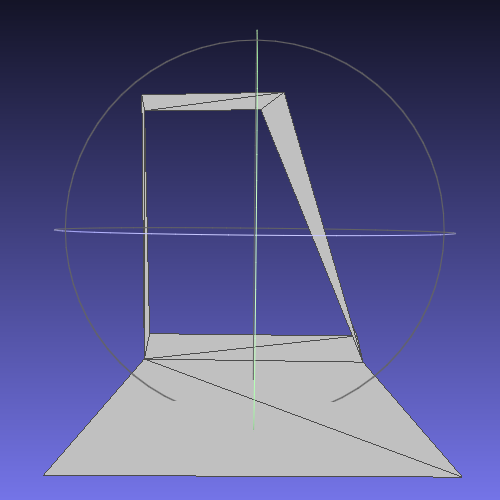
\includegraphics[height=4cm]{imagens/printResultadoDurerEsquerda.png}
					\label{resultadosDurer2}
				}
				\quad
				\subfloat[Reconstrução sob mesmo ponto de vista da cena da litografia de Dürer]{
					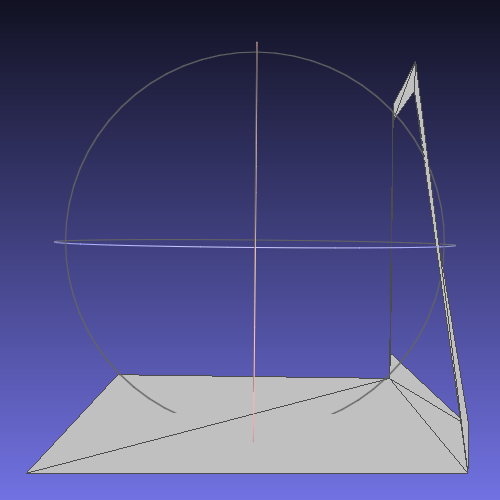
\includegraphics[height=4cm]{imagens/printResultadoDurerFrente.png}
					\label{resultadosDurer3}
				}
				\caption{A reconstrução da cena da litografia de Durer (Faces inseridas manualmente)}
				\label{resultadosDurerTriplo}
			\end{figure}
			
			No caso da litografia do Durer, o ponto de vista da imagem corrobora para uma melhor convergência de valores para coordenada Z. Todavia, a demarcação das referências e pontos de interesse é muito difícil dada a pequena região e ausência de dados claros sobre dimensões. Assim, o resultado da reconstrução sofre distorções causadas por má catalogação de dados iniciais.
			
			A imagem do Bule de Newell foi dispensada pois, dada a necessidade de demarcação de pontos de referência, esta não possibilitava um bom referenciamento (vide figura \ref{imagemBuleDispensada}) devido à ausência de pontos interessantes nessa região e o fato de sua projeção ser paralela, o que causaria a má calibração de câmera (que atende ao modelo em perspectiva).
			
			\begin{figure}[!htb]
				\centering
				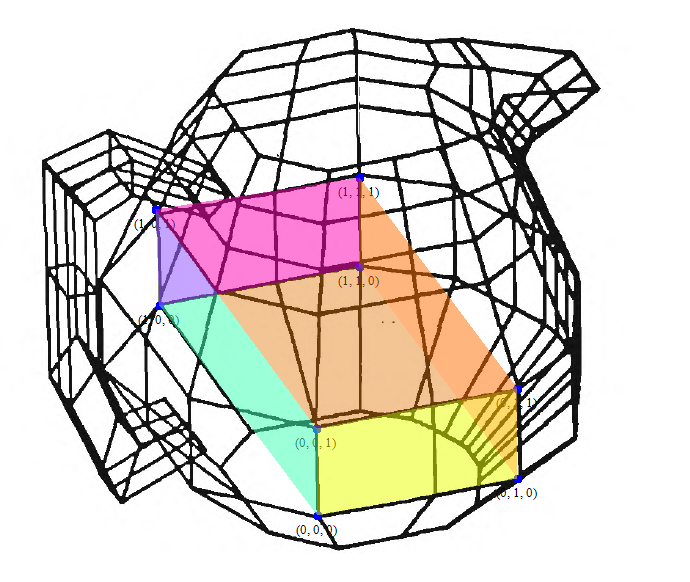
\includegraphics[height=8cm]{imagens/printBuleDispensada.png}
				\caption{Referenciamento na imagem do Bule de Newell}
				\label{imagemBuleDispensada}
			\end{figure}
			
			Os dados e resultados destas reconstruções estão disponíveis em \url{https://github.com/ivancezanne/TCC/tree/master/App_Reconstrucao/Resultados}.
			
		\section{Discussões}
			\label{secaoDiscussoes}
			
			Nota-se que há uma série de limitações à técnica de reconstrução que, ao fim, causa certa imprecisão ou restrição nos resultados objetivados. A delimitação de uma área de busca fixa, por exemplo, impede que um conjunto maior de reconstruções seja executado; a metodologia de demarcação - por \textit{clicks} - é costumeiramente imprecisa; e a estratégia de eliminação da multiplicidade projetiva não fora tão eficaz quanto o necessário.
			
			De qualquer forma, a exemplo da litografia do Dürer e da imagem do \textit{VW Beetle} de Sutherland, viu-se que as imagens não propiciaram uma boa catalogação de dados, uma vez que medidas eram inexistentes ou não correspondiam às medidas que o software requisitava; e, a exemplo da imagem do Bule de Newell, a isometria da projeção paralela impede o bom funcionamento da calibração de câmera necessária à reconstrução.
			
			Embora tenha-se notado que os dados utilizados para a reconstrução neste trabalho são insuficientes para uma reconstrução perfeita, pode-se concluir que o aprimoramento de uma técnica, baseada na descrita na seção \ref{appDeteccaoRetas}, de detecção de regiões de interesse parametrizáveis (retas, curvas ou superfícies) é uma promissora abordagem para uma reconstrução mais fiel dos objetos retratados; uma vez que restrições algébricas inerentes ao elemento geométrico detectado podem se aliar às restrições projetivas e resolver, com maior grau de verossimilhança, o problema da multiplicidade projetiva. Neste ínterim, condições de simetria e repetições seriam, também, melhor aplicáveis.
			
			Salienta-se, ainda, que o resultado gerado pelo \textit{software} de reconstrução é disponibilizado em arquivos de extensão PLY e, portanto, pode ser lido pelos principais programas de modelagem 3D; além disso, os \textit{softwares} anexos ao de reconstrução desempenham um bom auxílio a este último, o que faz deste trabalho um pacote contíguo de ferramentas computacionais direcionadas à reconstrução 3D.
			
			Em adição, é importante notar a importância deste trabalho na busca por uma expansão no rol de técnicas de reconstrução 3D, o qual ainda é muito baseado em técnicas de multivisão. 
			
			Por fim, nota-se que a técnica de reconstrução desenvolvida neste trabalho gera resultados, no mínimo, coesos e, dentro das limitações que esta veio a sofrer a fim de que seu desenvolvimento coubesse no prazo designado ao projeto, satisfaz uma necessidade inicial de obtenção de dados tridimensionais.
			
		\section{Trabalhos Futuros}
			\label{secaoTrabalhosFuturos}
			
			Como futura expansão deste trabalho está a já descrita integração da técnica de reconstrução com a de detecção de regiões descritíveis parametricamente. Além disso, focando o desenvolvimento desta técnica em um escopo mais específico, é possível obter melhor desempenho uma vez que, neste âmbito, a descrição prévia dos objetos reconstruídos seria facilitada e, portanto, mais rica.
			
			Especificamente, melhorar e aplicar esta técnica de reconstrução em retratos de modelos arquitetônicos, de forma similar a \cite{3DFromLineDrawings}, a fim de possibilitar um estudo de restauro e documentação patrimonial mais rico é o próximo intento.